\documentclass{article}


\include{stddefs}
\include{imodefs}

\newcommand{\stop}{\end{document}\bye}

\begin{document}


\chapterno{9}
\chapter{Convex optimization}

In this last chapter we will deal exclusively with convex optimization problems.

Recall that a convex optimization problem has the form

  \begin{align*}
    &\text{Minimize} &f(x_1, \dots, x_d)\\
    &\text{with constraint}\\
    &&(x_1, \dots, x_d)\in C,
  \end{align*}
  where $C\subseteq \RR^d$ is a \emph{convex subset} (see Definition \ref{Def:convexsubset}) and $f:C\rightarrow \RR$ a \emph{convex function} (see Definition \ref{Def:convexfunction}). We will mainly
  deal with the case, where $f$ is differentiable defined on all of $\RR^d$ in addition to just being convex defined on $C$. Also recall that convex optimization problems are very well behaved in the sense that local minima are global (see Theorem \ref{Thm:convexoptnice}).


  \begin{example}\label{firstexco}
    Below is an example of a convex optimization problem in the plane $\RR^2$.
    \begin{align*}
    &\text{Minimize} &x^2 + y^2\\
    &\text{with constraint}\\
    &&(x, y)\in C,
    \end{align*}
    where $C$ is the subset of points $(x, y)$ in $\RR^2$ satisfying
    \begin{align*}
      x + y &\geq 2\\
      y &\leq 2\\
      x &\leq 3\\
      y &\geq 1.
    \end{align*}
  \end{example}

  \beginshex
  Sketch the subset $C$ in Example \ref{firstexco}. Show that Example \ref{firstexco} really is a
  convex optimization problem and solve it.
  \endshex

  Below is an example of a convex optimization problem modelling the real life problem of placing a fire station (center of circle) so that the maximal distance to the surrounding houses (points to be enclosed) is minimal.

  \begin{example}\label{enclcircle}
    Given $n$ points
$(x_1, y_1), \dots, (x_n, y_n)\in \RR^2$, what is the center and
radius of the smallest circle containing these points?

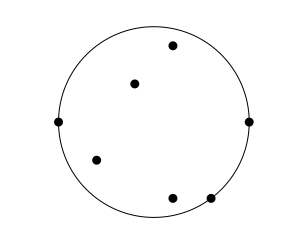
\includegraphics{mincircle.png}

We can write this optimization problem as
    \begin{align}\label{opt1}
    &\text{Minimize}\quad r\\
    &\text{with constraint}\\
    &&(x, y)\in C,
    \end{align}
    where
    $$
    C = \{(x, y)\in \RR^2 \mid (x - x_i)^2 + (y- y_i)^2 \leq r^2\quad\text{for}\quad i = 1, \dots, n\}.
    $$
    Upon rewriting this turns into the optimization problem
    \begin{align}\label{opt2}
    &\text{Minimize} &x^2 + y^2 + \lambda\\
    &\text{with constraint}\\
    &&(x, y)\in C',
    \end{align}
    where
    $$
    C' = \{(x, y)\in \RR^2 \mid x_i^2 + y_i^2 \leq 2 x_i x + 2 y_i y + \lambda\quad \text{for}\quad i = 1, \dots, n\}.
    $$
  \end{example}
  
  \beginshex
  Prove that \eqref{opt1} and \eqref{opt2} both are convex optimization problems.
  Explain how \eqref{opt1} is rewritten into \eqref{opt2}.

  \begin{hideinbutton}{Hint}
    Expand
    $$
    (x - x_i)^2 + (y- y_i)^2 \leq r^2
    $$
    and put $\lambda = r^2-x^2-y^2$.
  \end{hideinbutton}
  \endshex
  

  
  \section{Finding the best hyperplane separating data}

  In section \ref{sectperceptron} we were
  presented with labeled data
  \begin{equation}\label{sepdata}
  (v_1, y_1), \dots, (v_m, y_m),
  \end{equation}
  where $v_i\in \RR^d$ and $y_i = \pm 1$. The task at hand was to separate differently
  labeled data by a hyperplane $\alpha^T v + \beta = 0$, such that
  \begin{align}\label{psep}
    \alpha^T v_i + \beta &> 0\quad\text{if}\quad y_i = 1\\
    \alpha^T v_i + \beta &< 0\quad\text{if}\quad y_i = -1
  \end{align}
  for $i = 1, ,\dots, m$. 
Please browse back to section \ref{sec:mlds} for the definition of a hyperplane in $\RR^d$.

  If the data in \eqref{sepdata} can be separated according to
  \eqref{psep}, we may find a hyperplane $(\alpha^*)^T x + \beta^* = 0$,
  such that
  \begin{align}\label{psepone}
    (\alpha^*)^T v_i + \beta^* &\geq 1\quad\text{if}\quad y_i = 1\\
    (\alpha^*)^T v_i + \beta^* &\leq -1\quad\text{if}\quad y_i = -1.
  \end{align}

  \beginshex
  How do you go from \eqref{psep} to \eqref{psepone}?

  \begin{hideinbutton}{Hint}
    Suppose that 
\begin{align*}
    \alpha^T v_i + \beta &> 0\quad\text{if}\quad y_i = 1\\
    \alpha^T v_i + \beta &< 0\quad\text{if}\quad y_i = -1.
\end{align*}
Let
\begin{align*}
    m &= \min\{\alpha^T v_i + \beta \mid y_i = 1\}\\
    M &= \max\{\alpha^T v_i + \beta \mid y_i = -1\}.
\end{align*}
Show that $m > 0$ and $M < 0$. How can $m$ and $M$ be applied in
constructing $\alpha^*$ and $\beta^*$?
  \end{hideinbutton}

  \endshex
  
  What does best hyperplane mean in this setting? This is the one maximizing the width of the
  strip between the two labeled clusters.

  \begin{figure}
    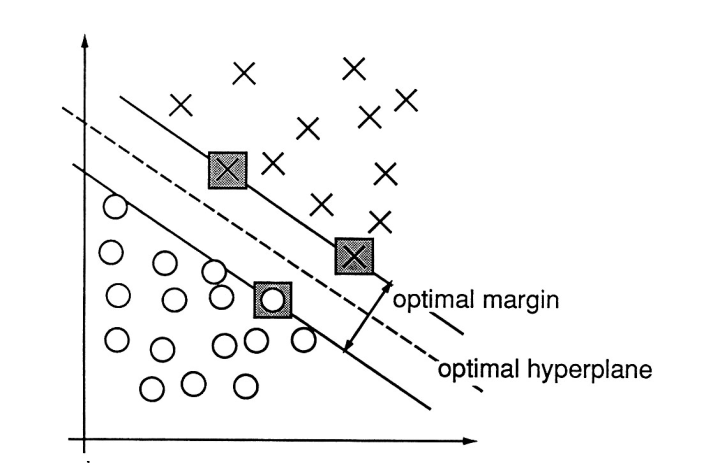
\includegraphics{Vapnik.png}
    \caption{Figure from the Cortes and Vapnik paper: \url{Support vector networks}{https://edtech.dk/IMO/img/cortes_vapnik95.pdf}, Machine Learning, 1995.}
  \end{figure}
  
  The distance from a hyperplane $\alpha^T v + \beta = 0$ to the positive labeled points is
  $$
  \min_{y_i = 1} \frac{\alpha^T v_i + \beta}{|\alpha|} = \frac{1}{|\alpha|}
  $$
  provided that the inequalities in \eqref{psepone} hold.

\beginshex
Let $H$ be the hyperplane in $\RR^d$ given by $\alpha^T x + \beta = 0$ and let $v\in \RR^d$.
The point closest to $v$ in $H$ can be found by solving the optimization problem
  \begin{align}\label{LagrH}
    &\text{Minimize} &|v - x|^2\\
    &\text{with constraint}\\
    &&x\in H.
  \end{align}

  Explain why \eqref{LagrH} is a convex optimization problem.
  
  Show how Theorem \ref{lagrmultthm} can be used to solve this optimization problem by
  first deducing the equations
  \begin{align}\label{equHL}
    -2(v - x) + \lambda \alpha &= 0\\
    \alpha^T x + \beta &= 0
  \end{align}
  for the Lagrange multiplier $\lambda$. Notice here that 
  $-2(v - x) + \lambda \alpha = 0$ above really contains $d$ equations, whereas
  $\alpha^T x + \beta = 0$ is only one equation in $x_1, \dots, x_d$, where
  $x = (x_1, \dots, x_d)^T$. Solve the equations \eqref{equHL} for $x\in \RR^d$ and $\lambda\in \RR$.
  How can we be sure that $x$ really is a minimum in
  \eqref{LagrH}?
  
  Finally show that the distance from $H$ to $v$ is given by the formula
  $$
  \left| \frac{\alpha^T v + \beta}{|\alpha|}\right|.
  $$
  \endshex
  

  The maximal width of the strip is then
  found by solving the convex optimization problem

    \begin{align} \label{sepoptpts}
    \text{Minimize}\qquad\quad &|\alpha|^2\\
     \text{with constraints}&\\
    \alpha^T v_i + \beta &\geq 1\quad\text{if}\quad y_i = 1\\
    \alpha^T v_i + \beta &\leq -1\quad\text{if}\quad y_i = -1.
  \end{align}

  \begin{example}
    Let us explicitly write up the optimization problem \eqref{sepoptpts} in
    a very simple situation: finding the best line $y = a x + b$ separating the points
    $(1, 1)$ and $(2, 2)$. In the notation of \eqref{psepone}, we have (without the
    stars on $\alpha$ and $\beta$)
    $$
    \alpha = \begin{pmatrix} a \\ -1 \end{pmatrix}\qquad\text{and}\qquad
    \beta = b
    $$
    so that
    $$
    \alpha^T \begin{pmatrix} x \\ y \end{pmatrix} + b = a x - y + b = 0.
    $$
    The points are
    $$
    v_1 = \begin{pmatrix} 1 \\ 1 \end{pmatrix}\qquad\text{and}\qquad
    v_2 = \begin{pmatrix} 2 \\ 2 \end{pmatrix},
    $$
    where $y_1 = 1$ and $y_2 = -1$.
    
    Therefore \eqref{sepoptpts} takes the form
  \begin{align}\label{concrsep}
 \text{Minimize}\qquad\quad &1 + a^2\\
     \text{with constraints}&\\
    a + b &\geq 2\\
    2 a + b&\leq 1
  \end{align}
  \end{example}

  \beginshex
  Solve the optimization problem \eqref{concrsep} and verify that the best line
  from the optimization problem is the one we expect it to be. Also, check how
  \url{WolframAlpha}{https://wolframalpha.com} solves this optimization problem.
  
  \begin{hideinbutton}{Hint}
    You could maybe use Fourier-Motzkin elimination to show that
    \begin{align*}
      a + b &\geq 2\\
    2 a + b&\leq 1
    \end{align*}
    implies $a \leq -1$.
  \end{hideinbutton}
  \endshex
  
  
  Notice that \eqref{sepoptpts} has number of constraints equal to the
  number of points to be separated. For an extended (soft margin)
  optimization problem, when the data at hand cannot be separated we
  refer to section 3 of the

    \url{Cortes and Vapnik  paper}{https://edtech.dk/IMO/img/cortes_vapnik95.pdf}.

  The vectors $v_i$ in the data set satisfying
  $$
    \alpha^T v_i + \beta = 1\qquad\text{or}\qquad\alpha^T v_i + \beta = -1
  $$
  are called \emph{support vectors} and the algorithms for solving \eqref{sepoptpts} are
  referred to as \emph{support vector machines}. 

Usually one does not use the optimization problem formulated in \eqref{sepoptpts}, but
rather its socalled (Lagrange) dual for finding the optimal hyperplane. This dual
optimization problem uses that $\alpha$ is a linear combination
\begin{equation}\label{lambdalc}
\alpha = \lambda_1 v_1 + \cdots + \lambda_m v_m
\end{equation}
of the support vectors. It is an optimization problem
in $\Lambda^T = (\lambda_1,\dots, \lambda_m)$
from \eqref{lambdalc} and looks like

    \begin{align} \label{sepoptptsdual}
    \text{Maximize}\qquad\quad &\lambda_1 + \cdots + \lambda_m - \frac{1}{2} \Lambda^T D \Lambda\\
     \text{with constraints}&\\
    \Lambda &\geq 0\\
    \Lambda^T Y &= 0,
    \end{align}
    where $Y =(y_1, \dots, y_m)^T$ is the vector of labels attached to
    the points $v_1, \dots, v_m$ and $D$ is the symmetric $m\times m$
    matrix given by
    \begin{equation}
    D_{ij} = y_i y_j\, v^T_i v_j = y_i y_j\, v_i\cdot v_j.
    \end{equation}

    The dual optimization problem \eqref{sepoptptsdual} can be derived
    formally from the original optimization problem
    \eqref{sepoptpts}. This is, however, beyond the scope of this
    course (see section 2.1 of the \url{Cortes and Vapnik paper}{https://edtech.dk/IMO/img/cortes_vapnik95.pdf}).

    
    \begin{example}\label{ex:cvxopt}
      Quadratic optimization problems, such as \eqref{sepoptpts} can in fact be handled by Sage (well, python
      in this case). See
      \url{CVXOPT}{https://cvxopt.org/index.html} for
      further information.  Note that the code below needs to be
      executed as \texttt{Python} code (choose Python in the pull
      down). It attempts (in general) to solve the optimization
      problem
      
    \begin{align*} 
    \text{Minimize}\qquad\quad &\frac{1}{2} x^T Q x + p^T x\\
     \text{with constraints}&\\
    G x &\leq h\\
    A x  &= b.
    \end{align*}


    
    In the Sage window below the optimization problem
\begin{align*} 
    \text{Minimize}\qquad\quad &2 x_1^2 + x_2^2 + x_1 x_2 + x_1 + x_2\\
  \text{with constraints}&\\
                               &x_1 \geq 0\\
                               &x_2 \geq 0\\
  &x_1 + x_2 = 1
    \end{align*}
    has been entered.
      
\begin{sage}
RealNumber=float
Integer=int

from cvxopt import matrix, solvers
Q = 2*matrix([ [2, .5], [.5, 1] ])
p = matrix([1.0, 1.0])
G = matrix([[-1.0,0.0],[0.0,-1.0]])
h = matrix([0.0,0.0])
A = matrix([[1.0], [1.0]])
b = matrix(1.0)
sol=solvers.qp(Q, p, G, h, A, b)
print(sol['x'])
\end{sage}

What happens if you remove
\begin{code}
RealNumber=float
Integer=int
\end{code}
from the code above?
\end{example}

\beginshex
Take a look at the input format in Example \ref{ex:cvxopt}. Can you tell which
optimization problem in this chapter is solved below? Also, the code below seems to report some errors after pressing the compute button. Can you make it run smoothly by making a very, very
small change?

\begin{sage}
from cvxopt import matrix, solvers
Q = 2*matrix([ [1.0, 0.0], [0.0, 0.0] ])
p = matrix([0.0, 0.0])
G = matrix([[-1.0,2.0],[-1.0,1.0]])
h = matrix([-2.0,1.0])
sol=solvers.qp(Q, p, G, h)
print(sol['x'])
\end{sage}
\endshex

  \subsection{Separating by non-linear functions}

  Sometimes one needs more complex separating curves than just a line. 
  Consider the five points
  $$
  (-1, 1), \quad (1, 1), \quad (1, -1), \quad (-1, -1),\quad \text{and} \quad (0, 0),
  $$
  where we wish to separate $(0, 0)$ from the other points. This is impossible
  using a line, but certainly doable by a circle
  \begin{equation}\label{circ}
  x^2 + y^2 = r^2,
  \end{equation}
  where $0<r<\sqrt{2}$:


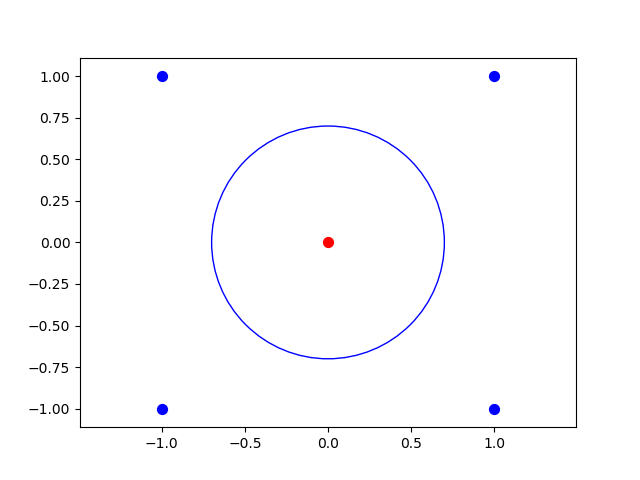
\includegraphics{simplesepcirc.png}

  The circle \eqref{circ} may be a circle in two
  dimensions, but viewed in three dimensions it turns into a
  hyperplane in the following way.

  By using the function $\varphi:\RR^2\rightarrow \RR^3$ given by
  $$
  \varphi(x, y) = (x^2, y^2, 1)\in \RR^3 = \{(x_1, y_1, z_1)\mid x_1, y_1, z_1\in \RR\},
  $$
  points lying on \eqref{circ} map to points lying on the
  hyperplane in $\RR^3$ given by
  $$
  x_1 + y_1 = r^2 z_1
  $$
  in $\RR^3$.
  
  
The general trick is to find a suitable map
$$
\varphi: \RR^d\rightarrow \RR^N,
$$
such that the transformed data
$$
  (\varphi(x_1), y_1), \dots, (\varphi(x_m), y_m)
  $$
  becomes linearly separable. 
  Since,
  $$
  \alpha = \lambda_1 \varphi(x_1) + \cdots + \lambda_m \varphi(x_m)
  $$
  for suitable $\lambda_1, \dots, \lambda_m\in \RR$, the (dual) optimization problem in  
\eqref{sepoptptsdual} becomes
    \begin{align*}
    \text{Maximize}\qquad\quad &\lambda_1 + \cdots + \lambda_m - \frac{1}{2} \Lambda^T D \Lambda\\
     \text{with constraints}&\\
    \Lambda &\geq 0\\
    \Lambda^T Y &= 0,
    \end{align*}
    where $Y =(y_1, \dots, y_m)^T$ is the vector of labels attached to
    the points $\varphi(x_1), \dots, \varphi(x_m)$ and $D$ is the symmetric $m\times m$
    matrix given by
    \begin{equation}\label{dmatrix}
    D_{ij} = y_i y_j\, \varphi(x_i)\cdot \varphi(x_j).
    \end{equation}

    The beauty of the dual problem is that we do not have to care about the (sometimes astronomical, even
    "infinite") dimension of $\RR^N$. The optimization problem is situated in $\RR^m$, where
    $m$ is the number of data points (or more precisely the number of constraints). We only need a clever way of getting our hands on
    $\varphi(x_i)\cdot \varphi(x_j)$ in \eqref{dmatrix}. Here an old concept from
    pure mathematics called kernels helps us.
  

    
\subsection{Kernels}
  
  A kernel is a function
  $k: \RR^n\times \RR^n \rightarrow \RR$, that is a hidden dot product
  in the following sense: there exists a function
  $$
  \varphi: \RR^n\rightarrow \RR^N,
  $$
  such that
    \begin{equation}\label{kerneq}
  k(u, v) = \varphi(u)\cdot \varphi(v).
\end{equation}

  \begin{example}\label{ex:kernel2}
    Let $k:\RR^2 \times \RR^2 \rightarrow \RR$ be given by
    $$
    k(u, v) = (u^T v + 1)^2.
    $$
    Then
    \begin{align}\label{polkernex}
      k((x_1, y_1), (x_2, y_2)) &= (x_1 x_2 + y_1 y_2 +1)^2\\
      &= x_1^2 x_2^2 + y_1^2 y_2^2 + 2 x_1 x_2 y_1 y_2 + 2 x_1 x_2 + 2 y_1 y_2 + 1.
    \end{align}
    One gleans from \eqref{polkernex} that $k$ is a kernel function, since \eqref{kerneq} is
    satisfied for $\varphi: \RR^2\rightarrow \RR^6$ given by
    $$
    \varphi(a, b) = (a^2, b^2, \sqrt{2} a b, \sqrt{2} a, \sqrt{2} b, 1).
    $$
  \end{example}


  \beginshex
  The simplest example of non-linear separation comes from the one dimensional case $\RR$:
  consider the labeled points $((-1), 1), ((1), -1), ((2), 1)$. Show by a drawing
  that these points cannot be separated in $\RR$, but that they become separable
  in $\RR^2$ by using $\varphi(x) = (x, x^2)$ i.e., that the labeled points
  $(\varphi(-1), 1), (\varphi(1), -1), (\varphi(2), 1)$ are linearly separable
  in $\RR^2$.
  
  How does one glean from \eqref{polkernex} that $k$ is a kernel function?
  \endshex
  
  Once we have a kernel for $\varphi$ we can replace the matrix in \eqref{dmatrix} by
  
    \begin{equation*}
    D_{ij} = y_i y_j\, k(x_i, x_j)
  \end{equation*}

  and proceed to solve the optimization problem without worrying about $\RR^N$ (or even an
  infinite dimensional space).

  \subsection{The kernel perceptron algorithm}

  Recall the stunningly simple perceptron algorithm from section
  \ref{sectperceptron}. This algorithm can be modified to handle
  non-linear separation too by using kernel functions. In fact, this
  modification was one of the inspirations for the development of the
  support vector machines described above.

  After having mapped a set of vectors $x_1, \dots, x_m\in \RR^d$ with
  labels $y_1, \dots, y_m\in\{\pm 1\}$ to
  $\varphi(x_1), \dots, \varphi(x_m)$, via $\varphi:\RR^d\rightarrow \RR^N$, we are looking for a vector
  $w\in \RR^N$, such that
  \begin{align}\label{rightperceptron}
    w^T \varphi(x_i) &> 0\quad\text{if}\quad y_i = 1\\
    w^T \varphi(x_i) &< 0\quad\text{if}\quad y_i = -1.
  \end{align}
  Such a vector is expressible as
  $$
  w = \lambda_1 \varphi(x_1) + \cdots + \lambda_m \varphi(x_m).
  $$
  The (dual) perceptron algorithm works adjusting the coefficients
  $\lambda_1, \dots, \lambda_m$ successively as follows: if
  $w^T$ is wrong about the placement of $\varphi(x_j)$ in \eqref{rightperceptron} i.e., 
  if $y_j w^T \varphi(x_j) < 0$, then let
  $$
  \lambda_j := \lambda_j + y_j.
  $$
  If we have a kernel function $k$ for $\varphi$, then
  $$
  w^T \varphi(x_j) = w\cdot \varphi(x_j) = \sum_{i=1}^m \lambda_i \varphi(x_i)\cdot \varphi(x_j) =
  \sum_{i=1}^m \lambda_i k(x_i, x_j)
  $$
  and we can use the kernel function in the algorithm without resorting to computing $\varphi$ and
  the inner product in $\RR^N$.

  \beginshex
  Use the kernel function in Example \ref{ex:kernel2} and the kernel perceptron algorithm to
  separate
  $$
  ((-1, -1), -1), \quad ((-1, 1), -1), \quad ((1, -1), -1), \quad ((0,0), 1), \quad ((1, 1), 1).
  $$
  Sketch the points and the separating curve.
  \endshex

  
  \section{Logarithmic barrier functions}

  We need an algorithm for solving optimization problems like \eqref{sepoptpts}.
  There is a very nice trick (probably going back to \url{von Neumann}{https://en.wikipedia.org/wiki/John_von_Neumann}) for solving constrained optimization problems of the form
  \begin{align}\label{ip:co}
    &\text{Minimize} &f(x_1, \dots, x_n)\\
    &\text{with constraint}\\
    &&(x_1, \dots, x_n)\in C,
  \end{align}
  where $C$ is defined by the differentiable functions
  $g_i:\RR^n\rightarrow \RR$ as
  $$
  C = \{x\in \RR^n \mid g_1(x) \leq 0, \dots, g_m(x)\leq 0\}.
  $$
  The functions $g_i$ define the boundary (or barrier) of $C$. We use
  them to define the logarithmic \emph{barrier function}
  $$
  B(x) = - \sum_{i=1}^m \log(-g_i(x))
  $$
  defined on the interior
  $$
  C^o = \{x\in \RR^n \mid g_1(x) < 0, \dots, g_m(x) < 0\}.
  $$
  The boundary of $C$ is
  $$
  \partial C = \{x\in C \mid g_1(x) = 0 \vee \cdots \vee g_m(x) = 0\}.
  $$
  You can see that the logarithmic barrier function explodes (becomes unbounded), when a
  vector $x\in C^o$ approaches $\partial C$, since $-\log(t)$ is unbounded as $t\to 0$ for $t>0$.

  The cool idea is  to consider the function
  \begin{equation}\label{barrier}
  f_\epsilon(x) = f(x) + \epsilon B(x)
  \end{equation}
  for $\epsilon > 0$. This function has a global minimum $x_\epsilon\in C^o$.

  \beginshex
  Prove that $f_\epsilon$ is a convex function if $f$ and $g_1, \dots, g_m$ are
  convex functions.
   
  \begin{hideinbutton}{Hint}
    Prove and use that if $f$ is a decreasing convex function (in one variable) and $g$ is a convex function, then
    $f(-g(x))$ is a convex function, where we assume the composition makes sense.
  \end{hideinbutton}
  \endshex
  
  The upshot is that $x_\epsilon \to x_0$ as $\epsilon\to 0$. This is the content of the following theorem, which we will not prove.

\begin{theorem}[emph]\label{thm:IPM}
  Let $x_\epsilon$ be a point in $C^o$ with
  \begin{equation*}
    f_\epsilon(x_\epsilon) = \min\left\{ f_\epsilon(x) \middle| x\in C^o \right\}
  \end{equation*}
  for $\epsilon > 0$ and $f^* = \min\left\{ f(x) \middle| x\in C \right\}$.  Then
  \begin{equation*}
    0\leq f(x_\varepsilon) - f^* \leq \varepsilon m
  \end{equation*}
  and $f(x_\varepsilon)\to f^*$ as $\varepsilon \to 0$. If
  \eqref{ip:co} has a unique optimum $x^*$, 
then by using $\epsilon=\frac1n$ we obtain a sequence $x_{\frac{1}{n}}\to  x^*$ as $n\to \infty$.
 \end{theorem}

 We move on to give concrete examples of Theorem \ref{thm:IPM} in action.
 
 \subsection{Quadratic function with polyhedral constraints}

 A much used setup in optimization is minimizing a quadratic functions
 subject to polyhedral constraints. This is the optimization problem
\begin{align}\label{qp}
  &\text{Minimize} &x^T Q x + c^T x\\
  &\text{with constraint}\\
  &&A x \leq b,
\end{align}
where $Q$ is an $n\times n$ matrix, $A$ is an $m\times n$ matrix,  $c\in \RR^n$ and $b\in \RR^m$.

Certainly the constraints $A x\leq b$ define a convex subset of $\RR^n$, but the function
$x^T Q x + c^T x$ is not strictly convex unless $Q$ is positive definite. If $Q$ is not
positive semidefinite \eqref{qp} is difficult.

If $Q$ is positive semidefinite, the interior point method outlined above usually works well.


\begin{example}
  The optimization problem \eqref{opt2} has the form \eqref{qp}, when we put
  \begin{align*}
    Q &=
        \begin{pmatrix}
          1 & 0 & 0\\
          0 & 1 & 0\\
          0 & 0 & 0
        \end{pmatrix}\\
    c &= \begin{pmatrix}
      0 \\ 0 \\ 2
    \end{pmatrix}\\
    A &=
        \begin{pmatrix}
          -2x_1 & -2y_1 & -1\\
          \vdots & \vdots & \vdots \\
          -2x_n & -2y_n & -1
        \end{pmatrix}\\
    b &= \begin{pmatrix}
      -x_1^2 - y_1^2\\
      \vdots \\
      -x_n^2 - y_n^2
      \end{pmatrix}
  \end{align*}
\end{example}

\begin{example}
  The optimization problem \eqref{sepoptpts} has the form \eqref{qp}, when we put
  \begin{align*}
    Q &=
        \begin{pmatrix}
          1 & 0 & \dots & 0 & 0\\
          0 & 1 & \dots & 0 & 0\\
          \vdots & \vdots &\ddots & \vdots\\
          0 & 0 & \dots & 1 & 0\\
          0 & 0 & \dots & 0 & 0
        \end{pmatrix}\\
    c &= \begin{pmatrix}
      0 \\ \vdots \\ 0
    \end{pmatrix}\\
    A &=
        \begin{pmatrix}
          -y_1 x_1 & -y_1\\
          \vdots & \vdots\\
          - y_n x_n & -y_n
        \end{pmatrix}\\
    b &= \begin{pmatrix}
      -1\\
      \vdots \\
      -1
      \end{pmatrix}
  \end{align*}
  Here $Q$ is a $(d+1)\times (d+1)$ matrix, $A$ is an $n\times (d+1)$ matrix and
  $b\in \RR^n$. 
\end{example}


Optimization of a quadratic function as in \eqref{qp} is implemented below using the
interior point method and \url{exact line search}{https://en.wikipedia.org/wiki/Line_search}. See Section 10.5.1 of my book \url{Undergraduate Convexity}{https://www.worldscientific.com/worldscibooks/10.1142/8527} for further details. Only
\texttt{python} with \texttt{numpy} is used.

\begin{sage}
import numpy as np

def Newton(Q0, c0, A0, b0, xinit, eps):

    nrows = len(A0)
    tolerance = 0.00001
    tolerancebisect = 0.0001

    
    Q = np.array(Q0)
    c = np.array(c0)
    A = np.array(A0)
    b = np.array(b0)
    x0 = np.array(xinit)

    def vabs(v): # Use L1 norm
      return sum(abs(x) for x in v)
    
    def tzero(x0, v):
        return min([(b[i] - A[i].dot(x0))/A[i].dot(v) for i in range(nrows) if A[i].dot(v)>0])

    recip = np.vectorize(lambda x: 1/x)
    
    def gradient(x):
      diff = b - A.dot(x)
      return 2*Q.dot(x) + c + (eps*recip(diff).dot(A))

    def hessian(x):
      diff = b - A.dot(x)
      return 2*Q + (eps*np.transpose(A).dot(np.diag(recip(np.multiply(diff, diff))).dot(A)))

    def g(t):
      return gradient(x0+t*v).dot(v)
  
    v = - np.linalg.inv(hessian(x0)).dot(gradient(x0))

    while(vabs(v) > tolerance):
        delta = tzero(x0, v)/2
        t1 = t2 = 0
        
        while (g(t2) < 0):
            t1 = t2
            t2 += delta
            delta /= 2

        crit = True
        while crit:
            t = t1 + delta
            if (g(t) < 0):
                t1 = t
            else:
                t2 = t
            delta /= 2
            crit = (delta > tolerancebisect) 
        
        x0 = x0 + (t*v)
        v = - np.linalg.inv(hessian(x0)).dot(gradient(x0))

    return x0

# Helper function for generating matrices for the optimization problem of finding
# the optimal hyperplane separating labeled points in the plane.
#
# Example:
#
# (Q1, c1, A1, b1) =
# bestsep([[1, 0], [2, 0], [3, 0], [3, 2],  [1, 1], [2, 2]], [1, 1, 1, 1, -1, -1], 10)
#
# generates data for separating ([1, 0], +1), ([2, 0], +1), ([3, 0], +1), ([3, 2), +1) from
# ([1, 1], -1), ([2, 2], -1)
#
# bounding the absolute value of the coordinates of alpha and beta by 10 (=bound).
#
# Note that it can be tricky to find x0 with A x0 < b1 as initial point. If this condition
# is broken, Newton fails.
#
# def bestsep(points, labels, bound):
#     A1 = [[-s*x, -s*y, -s] for ([x, y], s) in zip(points, labels)]
#     b1 = len(points)*[-1]
#     c1 = [0, 0, 0]
#     Q1 = [[1, 0, 0], [0, 1, 0], [0, 0, 0]]
#     A1 = [[1, 0, 0], [-1, 0, 0], [0, 1, 0], [0, -1, 0], [0, 0, 1], [0, 0, -1]] + A1
#     b1 = (6*[bound]) + b1
#     return (Q1, c1, A1, b1)
    


# Enclosing circle:
A1 = [
    [0, 0, 1],
    [0, 0,-1],
    [-4, -4, -1],
    [6, -4, -1],
    [-2, 0, -1],
    [4, -2, -1],
    [2, -6, -1],
    [0, -8, -1]
]

b1 = [20, 0, -8, -13, -1, -5, -10, -16]
Q1 = [[1, 0, 0], [0, 1, 0], [0, 0, 0]]
c1 = [0, 0, 1]
  
Newton(Q1, c1, A1, b1, [0,0,18], 0.0001)
\end{sage}


\begin{example}

  Below are samples of output running the interior point algorithm on the enclosing circle problem in Example \ref{enclcircle}.

  $$
  \epsilon = 1,\quad 0.5, \quad 0.1, \quad 0.05, \quad 0.01, \quad 0.005, \quad 0.001, \quad 0.0005, \quad 0.0001
  $$
  in the barrier function $f_\epsilon(x)$ in \eqref{barrier}. We are attempting to compute the center
  of the smallest enclosing circle of the points
  $$
  (0, 0), \quad (2,2), \quad (-3, 2), \quad (1, 0), \quad (-2, 1), \quad (-1, 3), \quad\text{and}\quad
  (0, 4).
  $$
\begin{code}
>>> Newton(Q1, c1, A1, b1, [0,0,18], 1)
array([-0.43814179,  1.84835643,  7.69779763])
>>> Newton(Q1, c1, A1, b1, [0,0,18], 0.5)
array([-0.45244596,  1.81135335,  4.99353576])
>>> Newton(Q1, c1, A1, b1, [0,0,18], 0.1)
array([-0.49569549,  1.84020923,  2.91071666])
>>> Newton(Q1, c1, A1, b1, [0,0,18], 0.05)
array([-0.49875614,  1.87002433,  2.63917096])
>>> Newton(Q1, c1, A1, b1, [0,0,18], 0.01)
array([-0.4999099 ,  1.93327221,  2.28805064])
>>> Newton(Q1, c1, A1, b1, [0,0,18], 0.005)
array([-0.49996901,  1.95176304,  2.20331123])
>>> Newton(Q1, c1, A1, b1, [0,0,18], 0.001)
array([-0.49999729,  1.97792915,  2.09031159])
>>> Newton(Q1, c1, A1, b1, [0,0,18], 0.0005)
array([-0.49999904,  1.98432672,  2.06370265])
>>> Newton(Q1, c1, A1, b1, [0,0,18], 0.0001)
array([-0.49999991,  1.99295433,  2.0283835 ])
\end{code}
The first two coordinates of the output are the $x$- and $y$-coordinates of the center. The third
is $\lambda$ from \eqref{opt2}. 
\end{example}

\beginshex
Try out the code in the Sage window above on the Exercises \ref{calcopt1}, \ref{calcopt2} and
\ref{calcopt3}. Check the output of the code by actually solving these exercises.
\endshex

\beginshex
Compute the best line separating the labeled data
\begin{code}
((1, 0), +1), ((2, 0), +1), ((3, 0), +1), ((3, 2), +1), ((1, 1), -1), ((2, 2), -1).
\end{code}
\endshex






\section{A geometric optimality criterion}

Consider the general optimization problem
  \begin{align}\label{co}
    &\text{Minimize} &f(x_1, \dots, x_n)\\
    &\text{with constraint}\\
    &&(x_1, \dots, x_n)\in C,
  \end{align}
  where $C$ is a subset of $\RR^n$.

  
  \begin{proposition}[emph]\label{simpopt}
  Suppose that $C\subseteq \RR^n$ is a convex subset and $f:\RR^n\rightarrow \RR$ a
  differentiable function in \eqref{co}. If $x_0\in C$ is an optimal solution of \eqref{co},
  then
  \begin{equation}\label{convecrit}
    \nabla f (x_0) (x - x_0) \geq 0\qquad\text{for every } x\in C.
  \end{equation}
  If $f$ in addition is a convex function, then \eqref{convecrit} implies that
  $x_0$ is optimal.
\end{proposition}
\begin{hideinbutton}{Proof}
  If $x_0$ is an optimal solution and $x\in C\setminus\{x_0\}$, then
  \begin{align*}
    0 &\leq f((1-t)x_0 + t x) - f(x_0) = f(x_0 + t(x-x_0)) - f(x_0)\\
    &= t\,\left (\nabla f(x_0)(x-x_0) + \epsilon(t (x-x_0)) \abs{x-x_0 }\right)
  \end{align*}
  for every $t$ with $0\leq t \leq 1$, where $\epsilon$ denotes the
  epsilon function in the definition of differentiability (see
  Definition \ref{diffdef}). Therefore
  \begin{equation*}
    \nabla f(x_0)(x-x_0) + \epsilon(t (x-x_0)) \abs{ x-x_0 }\geq 0
  \end{equation*}
  for $0\leq t\leq 1$. This is only possible if $\nabla
  f(x_0)(x-x_0)\geq 0$.  We have silently applied the convexity of $C$
  and the differentiability of $f$ at $x_0$.

  If $f$ in addition is convex and \eqref{convecrit} holds, then
  Theorem \ref{thmdiffsubdif} shows that $x_0$ is an optimal solution.
\end{hideinbutton}


\begin{example}

A nice application of Proposition \ref{simpopt} is for example to the optimization problem

\begin{align*}
    &\text{Minimize} &(x+1)^2 + (y+1)^2\\
    &\text{with constraint}\\
    &&x^2 + 3 y^2 \leq 1
\end{align*}

Here Proposition \ref{simpopt} shows that $x_0=\left(-\tfrac{1}{2}, -\tfrac{1}{2}\right)$ is optimal, since
the hyperplane
$$
\nabla f(x_0) x = \nabla f(x_0) x_0
$$
touches the boundary of
$$
C = \{(x, y)\in \RR^2\mid x^2 + 3y^2\leq 1\}
$$
as shown below.


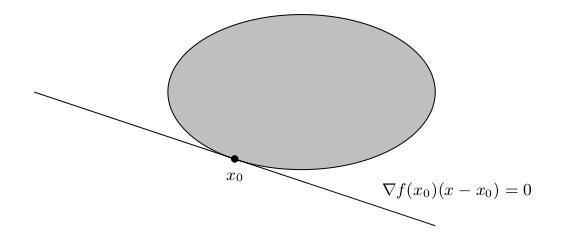
\includegraphics{simpopt.png}



\end{example}


\newcommand{\Set}[2]{\left\{ #1 \middle| #2 \right\}}


\beginshex
Sketch how Proposition \ref{simpopt} applies to show that an optimum in a linear programming
problem
\begin{align*}
    &\text{Minimize} &c x + d y\\
    &\text{with constraint}\\
    &&A \begin{pmatrix} x \\ y \end{pmatrix} \leq b
  \end{align*}
in the plane $\RR^2$ always can be found in a vertex.
\endshex

\beginshex
  Let $f:\RR^2\rightarrow \RR$ be a differentiable convex function and
  \begin{equation*}
    S =\Set{ (x, y) }{ -1 \leq x \leq 2, -1 \leq y \leq 1 }.
  \end{equation*}
  Suppose that $\nabla f(x_0) = (1,0)$ for $x_0 =
  (-1,\frac{1}{2})$. Prove that $x_0$ is a minimum for $f$ defined on
  $S$.
\endshex

\beginshex
  Guess the solution to the optimization problem
  \begin{equation*}
    \min\Set{ (x-5)^2 + (y-5)^2\, }{ \, x\geq 0,\, y\geq 0,\, x^2 +
      y^2 \leq 25 }. 
  \end{equation*}
  Show that your guess was correct!
\endshex



\section{KKT}

The KKT in the title of this section is short for Karush-Kuhn-Tucker.

We will limit ourselves to a convex optimization problem of the form
  \begin{align}\label{cokkt}
    &\text{Minimize} &f(x_1, \dots, x_n)\\
    &\text{with constraint}\\
    &&(x_1, \dots, x_n)\in C,
  \end{align}
  where $C$ is defined by the differentiable convex functions
  $g_i:\RR^n\rightarrow \RR$ as
  $$
  C = \{v\in \RR^n \mid g_1(v) \leq 0, \dots, g_m(v)\leq 0\}
  $$
  and $f:\RR^n\rightarrow \RR$ is a convex function.

  To the optimization problem \eqref{cokkt} we associate the (famous)
  \url{Karush-Kuhn-Tucker}{https://en.wikipedia.org/wiki/Karush\%E2\%80\%93Kuhn\%E2\%80\%93Tucker_conditions} (KKT) conditions:
  \begin{align}[emph]\label{kktcond}
    &\lambda_1 \geq 0, \dots, \lambda_m\geq 0\\
    \\
    &g_1(v_0)\leq 0, \dots, g_m(v_0)\leq 0\\
    \\
    &\lambda_1 g_1(v_0) = 0, \dots, \lambda_m g_m(v_0) = 0\\
      \\
    &\nabla f(v_0) + \lambda_1 \nabla g_1(v_0) + \cdots + \lambda_m
    \nabla g_m(v_0) = 0.
  \end{align}

  Notice that the KKT conditions consist of  $2m$ inequalities and $m+n$
  equations in the $m+n$ unknowns
  $\lambda_1, \dots, \lambda_m, v_0 = (x_1, \dots, x_n)$. The KKT
  conditions form a surprising theoretical foundation for optimization
  problems of the type in \eqref{cokkt}. You should take a peek back
  to the theory of Lagrange multipliers in section \ref{Lagrangemult} and
  compare with \eqref{kktcond}.

  \begin{example}\label{KKTcondsex}
    The KKT conditions associated with the convex optimization problem in \eqref{firstexco} are
    \begin{align*}
      \lambda_1, \lambda_2, \lambda_3, \lambda_4 & \geq 0\\
 -x -y + 2 &\leq 0\\
  y - 2&\leq 0\\
  x - 3&\leq 0\\
  -y + 1 &\leq 0\\
  \lambda_1 (- x - y + 2) &=0\\
  \lambda_2 (y - 2) &= 0\\
  \lambda_3 (x - 3) &= 0\\
  \lambda_4 (-y + 1) &= 0\\
  2 x - \lambda_1  + \lambda_3 &= 0\\
  2 y - \lambda_1  + \lambda_2 -\lambda_4 &= 0.
\end{align*}
    
  \end{example}

  \beginshex
  Verify that the KKT conditions of the optimization problem in \eqref{firstexco} are the
  ones given in Example \ref{KKTcondsex}.
  \endshex

To state our main theorem we
  need a definition.

\begin{definition}[emph]
  The optimization problem \eqref{cokkt} is called \emph{strictly
    feasible} if there exists $z_0\in \RR^n$ with
  \begin{align*}
    g_1(z_0) &< 0\\
    &\vdots\\
    g_m(z_0) &< 0.
  \end{align*}
\end{definition}

Below is the main result in our limited convex setting. We will not go into the proof, which can be found in my book \url{Undergraduate Convexity}{https://www.worldscientific.com/worldscibooks/10.1142/8527}.

\begin{theorem}[emph]\label{thmKKT}
\begin{enumerate}[(i)]
\item
  Let $v_0$ be an optimal solution of \eqref{cokkt}. If \eqref{cokkt}
  is strictly feasible, then the KKT conditions are satisfied at $v_0$
  for suitable $\lambda_1, \dots, \lambda_m$.
\item
  If the KKT conditions are satisfied at $z\in \RR^n$ for some
  $\lambda_1, \dots, \lambda_m$, then $z$ is an optimal solution to
  \eqref{cokkt}.
  \end{enumerate}
\end{theorem}




\newcommand{\qtextq}[1]{\quad\text{#1}\quad}



\section{Computing with KKT}

\subsection{Strategy}

A general strategy for finding solutions to the KKT conditions in \eqref{kktcond}
is zooming in on (the Lagrange multipliers) $\lambda_1, \dots, \lambda_m$ testing
each of them for the two cases $\lambda_i = 0$ and $\lambda_i> 0$.

One important point, which you can read from \eqref{kktcond}, is
that $g_i(v_0) = 0$ if $\lambda_i > 0$. To further elaborate, if
$\lambda_i > 0$, then an optimal solution must satisfy $g_i(v_0) = 0$.

\beginshex
So where exactly in \eqref{kktcond} is the above claim verified?
\endshex

The condition $\lambda_i = 0$ simplifies the equations
$$
\nabla f(v_0) + \lambda_1 \nabla g_1(v_0) + \cdots + \lambda_m
    \nabla g_m(v_0) = 0
$$
in \eqref{kktcond}.    

In principle to solve the KKT conditions, one has to try out all the
$2^m$ possibilities coming from $\lambda_i = 0$ or $\lambda_i > 0$ for $i=1, \dots, m$.

\beginshex
Why $2^m$ possibilities above?
\endshex

\beginshex
How do you solve the optimization problem (or decide there is no solution)
if $\lambda_1 = \cdots = \lambda_m = 0$?
\endshex



\subsection{Example}

Let $C$ denote the set
(see Figure \ref{fig:KKTexample}) of points $(x, y)\in \RR^2$ with
\begin{align*}
  x^2 + 2y^2 &\leq 1\\
  x + y &\leq 1\\
  y &\leq x.
\end{align*}
We will illustrate the mechanics of solving the KKT conditions in
finding an optimal solution for
  \begin{align}\label{eq:KKTex}
    &\text{Minimize} &x + 3 y\\
    &\text{with constraint}\\
    &&(x, y)\in C.
  \end{align}

\begin{figure}\label{fig:KKTexample}
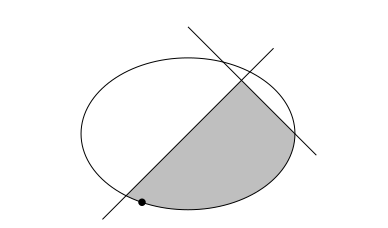
\includegraphics{kktexample.png}
  \caption{The convex set $C$ with optimal solution for
    \eqref{eq:KKTex} marked.}
\end{figure}

Putting
\begin{align*}
  g_1(x, y) &= x^2 + 2 y^2 -1\\
  g_2(x, y) &= x + y  - 1\\
  g_3(x, y) &= y - x
\end{align*}
and $f(x, y) = x + 3y$, we are in a position to apply Theorem
\ref{thmKKT}, since $g_1, g_2, g_3$ are convex functions and
$g_1(z_0) < 0, g_2(z_0)<0, g_3(z_0)<0$ for $z_0 = (0,
-\frac{1}{2})$. This means that an optimal solution of
\eqref{eq:KKTex} satisfies the KKT conditions. The same theorem tells
us that the $x_0$ in a solution of the KKT conditions is an optimal
solution (here we also use that $f$ is a convex function). The full
set of KKT conditions in
$x, y, \lambda_1, \lambda_2, \lambda_3\in \RR$ are
\begin{align*}
  x^2 + 2y^2 -1 &\leq 0\\
  x + y -1&\leq 0\\
  y - x&\leq 0\\
  \lambda_1, \lambda_2, \lambda_3 & \geq 0\\
  \lambda_1 (x^2 + 2y^2 -1) &=0\\
  \lambda_2 (x+y -1) &= 0\\
  \lambda_3 (-x + y) &= 0\\
  1 + 2 \lambda_1 x + \lambda_2 - \lambda_3 &= 0\\
  3 + 4\lambda_1 y + \lambda_2 +\lambda_3 &= 0.
\end{align*}
A strategy for finding a solution to the KKT conditions is trying (the
eight) different combinations of strict inequalities in $\lambda_1,
\lambda_2, \lambda_3\geq 0$. You can see from the last two equations
that $\lambda_1 = 0$ is impossible. The condition $\lambda_1 > 0$
shows that an optimal solution has to occur on the lower arc in
Figure \ref{fig:KKTexample}. If $\lambda_3 > 0$, then $x = y$ and
$\lambda_2 = 1+3 \lambda_3 > 0$ by the last two equations. This
implies $x = y = \frac{1}{2}$ violating $x^2 + 2 y^2 - 1 =
0$. Therefore $\lambda_3 = 0$. If $\lambda_2 > 0$, then $y=1-x$ and $5
+ 4 \lambda_1 + 3 \lambda_2 = 0$ by $\lambda_3 = 0$ and the last two
equations. Therefore $\lambda_2=0$. So we are left with the case
$\lambda_1 > 0$ and $\lambda_2 = \lambda_3 = 0$ giving
\begin{equation*}
  x = -\frac{1}{2\lambda_1}\qtextq{and}   y = -\frac{3}{4 \lambda_1}.
\end{equation*}
Inserting this into $x^2 + 2 y^2 - 1 = 0$ we end up with (see
Figure \ref{fig:KKTexample})
\begin{equation*}
  \lambda_1 = \frac{\sqrt{11}}{2 \sqrt{2}},\quad x =
  -\sqrt{\frac{2}{11}}
  \qtextq{and} y = -\frac{3}{\sqrt{22}}.
\end{equation*}

Theorem \ref{thmKKT} is beautiful mathematics. Going through the KKT
conditions as above can be quite lengthy if not impossible in
practice. As we have seen, there are other methods for (at least)
approximating an optimal solution.


\section{Optimization exercises}

Below are some exercises especially related to the KKT conditions. In some of the
exercises the minimization problem
  \begin{align}
    &\text{Minimize} &f(x_1, \dots, x_n)\\
    &\text{with constraint}\\
    &&(x_1, \dots, x_n)\in C,
  \end{align}
  is denoted
  $$
  \min\{f(x_1, \dots, x_n) \mid (x_1, \dots, x_n)\in C\}.
  $$
This should cause no confusion.
  
\beginshex

Consider the optimization problem

  \begin{align}\label{optokt13}
    &\text{Minimize} &-x + y\\
    &\text{with constraints}\\
    &&x^2  +y^2 &\leq 1\\
    &&(x+1)^2 + (y-1)^2&\leq 1
  \end{align}

  \begin{enumerate}[(a)]
  \item
    Show that \eqref{optokt13} is a convex optimization problem.
\item
  Sketch the set of constraints in $\RR^2$ and show that $\left(-\frac{1}{2}, \frac{1}{2}\right)$ cannot be an optimal
  solution to \eqref{optokt13}.
\item
  Write up the KKT conditions for \eqref{optokt13} and explain theoretically (without actually solving them) why
  they must have a solution.
  \item
    Now solve \eqref{optokt13}. Is the solution unique?
\end{enumerate}


\endshex


\beginshex

Consider the function $f:\RR^3\rightarrow \RR$ given by
$$
f(x_1, x_2, x_3) = 2 x_1^2 + 3 x_2^2 + 4 x_3^2.
$$

\begin{enumerate}[(a)]
\item
  Show that $f$ is strictly convex.
\item
Let $S \subseteq \RR^3$ denote the subset of points $(x_1, x_2, x_3)\in \RR^3$ satisfying
\begin{align*}
x_1 + x_2 + x_3 &\geq 1\\
x_1 + 2 x_2 + 3 x_3 &\leq 5
\end{align*}
Show that $S$ is a closed convex subset.
\item
Solve the optimization problem
  \begin{align}\label{optokt13}
    &\text{Minimize} &f(x_1, x_2, x_3)\\
    &\text{with constraints}\\
    &&(x_1, x_2, x_3)\in S
  \end{align}
\end{enumerate}
\endshex

\beginshex

Let $S\subseteq B \subseteq \RR^3$, where 
\begin{align*}
S &= \{(x, y, z)\in \RR^3 \mid x^2 + y^2 + z^2 = 1\}\qquad\text{and}\\
B &= \{(x, y, z)\in \RR^3 \mid x^2 + y^2 + z^2 \leq 1\}.
\end{align*}


\begin{enumerate}[(a)]
\item
  Why does the optimization problem

  \begin{align}\label{optokt14}
    &\text{Minimize} &x + 2y + z\\
    &\text{with constraints}\\
    &&(x, y, z)\in S
\end{align}
have a solution?
\item
Find all optimal solutions to \eqref{optokt14}.  
\item
Let $a, b, c\in \RR$, where at least one of $a, b, c$ is non-zero. Show that an optimal solution to
  \begin{align*}
    &\text{Minimize} &a x + b y + c z\\
    &\text{with constraints}\\
    &&(x, y, z)\in B
\end{align*}
belongs to $S$.
\end{enumerate}
\endshex



\beginshex

  Let
  \begin{equation*}
    S = \Set{ (x, y)\in \RR^2 }{
      \begin{matrix}
        -x  & - & y   & \leq & 0 \\
        2 x & - & y   & \leq & 1 \\
        -x & + & 2 y & \leq & 1
      \end{matrix}
    }.
  \end{equation*}
  \begin{enumerate}
  \item Use the KKT conditions to solve the minimization problem
    \begin{equation*}
      \min\Set{ -x - 4 y }{(x, y)\in S }.
    \end{equation*} 

  \item Use the KKT conditions to solve the minimization problem
    \begin{equation*}
      \min\Set{ x + y }{ (x, y)\in S }.
    \end{equation*} 
  \end{enumerate}
\endshex

\beginshex
  Solve the optimization problem
  \begin{equation*}
    \min\Set{x^2 + 2 y^2 + 3 z^2- 2 x z - x y}{
      \begin{matrix}
        2x^2 + y^2 + z^2 & \leq & 4 \\
        1 & \geq & x+y+z
      \end{matrix}
    }.
  \end{equation*}
  \endshex

  \beginshex
  
  Let $S =\Set{ (x, y) }{ 2 x^2 + y^2 \leq 3, \, x^2 + 2y^2 \leq 3 }$
  and $f(x, y) = (x-4)^2 + (y-4)^2$.
  \begin{enumerate}
  \item State the KKT conditions for $\min\Set{ f(x, y) }{ (x, y)\in S
    }$ for $(x, y) = (1,1)$.
  \item Suppose now that $g(x, y) = (x-a)^2 + (y-b)^2$. For which $a$
    and $b$ does $\min\Set{ g(x, y) }{ (x, y)\in S }$ have optimum in
    $(1,1)$?  State the KKT conditions when $(a, b) = (1,1)$.
  \end{enumerate}
\endshex


\beginshex

  Let $f:\RR^2\rightarrow \RR$ be given by
  \begin{equation*}
    f(x, y) = (x-1)^2+ (y-1)^2 + 2 x y.
  \end{equation*}
  \begin{enumerate}
  \item Show that $f$ is a convex function.

  \item Find $\min\Set{ f(x, y) }{ (x, y)\in \RR^2 }$. Is this minimum
    unique?  Is $f$ a strictly convex function.

    Let
    \begin{equation*}
      S = \Set{ (x, y)\in \RR^2 }{
        x + y \leq 0, \quad x - y \leq 0
      }.
    \end{equation*}
  \item Apply the KKT-conditions to decide if $(-1, -1)$ is an optimal
    solution to
    \begin{equation*}
      \min\Set{ f(x, y) }{ (x, y)\in S }.
    \end{equation*} 
  \item Find
    \begin{equation*}
      m = \min\Set{ f(x, y) }{ (x, y)\in S }
    \end{equation*}
    and
    \begin{equation*}
      \Set{ (x, y)\in \RR^2 }{ f(x, y) = m }.
    \end{equation*}
  \end{enumerate}
\endshex

\beginshex

  Let $f:\RR^2\rightarrow \RR$ be given by
  \begin{equation*}
    f(x, y) = x^2 + y^2 - e^{x-y-1}
  \end{equation*}
  and let
  \begin{equation*}
    C =\Set{ (x, y) }{ x - y \leq 0 }.
  \end{equation*}
  \begin{enumerate}
  \item Show that $f:\RR^2\rightarrow \RR$ is not a convex function.
  \item Show that $f$ is a convex function on the open subset
    \begin{equation*}
      \Set{ (x, y) \in \RR^2 }{ x - y< \tfrac{1}{2} }
    \end{equation*}
    and conclude that $f$ is convex on $C$.
  \item Show that $v = (0,0)$ is an optimal solution for the
    optimization problem $\min\Set{ f(v) }{ v\in C }$. Is $v$ a unique
    optimal solution here?
  \end{enumerate}
\endshex

\beginshex

  Let $f:\RR^4\rightarrow \RR$ be given by
  \begin{equation*}
    f(x_1, x_2, x_3, x_4) = (x_1 - x_3)^2 + (x_2 - x_4)^2
  \end{equation*}
  and $C\subseteq \RR^4$ by
  \begin{equation*}
    C =\Set{ (x_1, x_2, x_3, x_4)\in \RR^4 }{ x_1^2 + (x_2 - 2)^2 \leq 1,\,
      x_3 -x_4\geq 0 }.
  \end{equation*}
  \begin{enumerate}
  \item Show that $f$ is a convex function. Is $f$ strictly convex?
  \item Show that $C$ is a convex subset of $\RR^4$.
  \item Does there exist an optimal point $v = (x_1, x_2, x_3, x_4)\in
    \RR^4$ for the minimization problem
    \begin{equation*}
      \min_{v\in C} f(v)
    \end{equation*}
    with $x_3 = x_4 = 0$?
  \item Does there exist an optimal point $v = (x_1, x_2, x_3, x_4)\in
    \RR^4$ for the minimization problem
    \begin{equation*}
      \min_{v\in C} f(v)
    \end{equation*}
    with $x_3 = x_4 = 1$?
  \end{enumerate}
\endshex



\beginshex

  Let
  \begin{equation*}
    f(x, y) = (x-1)^2 + y^2
  \end{equation*}
  and
  \begin{equation*}
    C =\Set{ (x, y)\in \RR^2 }{ -1\leq x \leq 0,\,\, -1 \leq y \leq 1 }.
  \end{equation*}
Solve the optimization problem
    \begin{equation*}
      \min\Set{ f(x, y) }{ (x, y)\in C }.
    \end{equation*}

\endshex

\beginshex

  Let $f:\RR^2\rightarrow \RR$ be given by
  \begin{equation*}
    f(x, y) = \tfrac{1}{2} x^2+ y^2-2 y+2.
  \end{equation*}
  Below, the minimization problem
  \begin{equation}\label{mini}
    \min\Set{ f(x, y) }{ (x, y) \in S }
  \end{equation}
  is analyzed for various subsets $S\subseteq \RR^2$.
  \begin{enumerate}
  \item Show that $f$ is a convex function
  \item \label{opg1} Let
    \begin{equation*}
      S =\Set{ (x, y)\in \RR^2 }{ - x + 2y \leq 1 }.
    \end{equation*}
    Show that $(-1, 0)\in S$ cannot be an optimal solution to
    \eqref{mini}. Find an optimal solution to \eqref{mini}.

  \item\label{opg2} Find an optimal solution in \eqref{mini} for
    \begin{equation*}
      S =\Set{ (x, y)\in \RR^2 }{ -x + 2y \geq 1 }.
    \end{equation*}
  \item Are the optimal solutions in \ref{opg1} and \ref{opg2} unique?
  \end{enumerate}
  \endshex

  
  \beginshex
  
  Let $f:\RR^2\rightarrow \RR$ be given by
  \begin{equation*}
    f(x, y) = 2x^2 +3 x + y^2 + y.
  \end{equation*}
  \begin{enumerate}
  \item Show that $f$ is a convex function and solve the minimization
    problem $\min\Set{ f(x, y) }{ x, y\in \RR }$.

    Now let
    \begin{equation*}
      S = \Set{ (x, y)\in \RR^2 }{
        \begin{matrix}
          x^2 +  (y+1)^2 & \leq & 1 \\
          y  -  x & \leq & 0
        \end{matrix}
      }
    \end{equation*}
    and consider the minimization problem (P) given by
    \begin{equation*}
      \min\Set{ f(x, y) }{ (x, y)\in S }.
    \end{equation*}

  \item Show using the KKT conditions that $(0,0)$ is not optimal for
    (P).

  \item Find an optimal solution for (P). Is it unique?
  \end{enumerate}
\endshex


\end{document}
